\chapter[Diversion Detection]{Diversion Detection}

The second aspect of this work is identifying potential places for diversion in a generic pyroprocessing facility. We took 2 primary approaches for this work, applying
a cumulative sum detection algorithm and performing sensitivity analysis on key facility parameters. 
\section{Cumulative Sum}

\subsection{Requirements of Diversion Detection}


The cumulative sum method (CUSUM) applied to Pyre was chosen to fit the following requirements: function with minimal prior information, have online diversion detection
capabilities, and fit a modular approach. The CUSUM change detection algorithm relies on developing an expected mean value of a data stream as shown by the following equations \cite{basseville_detection_1993}.

\[ f_{t+1} = max(0, f_t + x_t - \mu - \delta) \]

Where:
\[ x_t = observed \hspace{2mm} data \]
\[ \mu = approximated \hspace{2mm} mean \]
\[ \delta = acceptable \hspace{2mm} change \]

This general function adds new observed values to the calculated mean. If the value is within region of error, typically 3$\sigma$, change is not reported. 
We favor this online diversion detection capability in an effort to achieve timely detection goals set by the IAEA \cite{international_atomic_energy_agency_implications_2004}.
These intermittent inspections only have access to portions of the complete data stream, thus we aim to mimic reality as closely as possible. In addition, we need this
algorithm to work on a variety of facilities with different sub-processes active, ruling out a nodal approach seen by \cite{Yilmaz_2016}.

\subsection{Limitations of selected method}

This approach is not without its drawbacks, since there is no prior data assumed we must generate a reasonable mean before being able to detect diversion. For this work
we assume a startup time of approximately 6 months before an appropriate mean can be developed. The next limitation faced with this approach is observing one data stream at a time, while
real inspections take a wide range of conditions into account. This concern is addressed by using sensitivity analysis, as seen later in this chapter, to inform on the most crucial
sub-processes or settings. 

CUSUM relies on a variable mean and noise to obscure possible change points. When a simulator knows the exact value at each time step, without human reporting or measurement error, change 
detection becomes trivial. To combat this issue, noise is artificially created when the CUSUM class reads data. This way \Cyclus retains its constant operating value while the change point
has potential to be obscured by measurement error. These detector uncertainties are assumed from common non-destructive and destructive assay practices used by the SEE LANL course \cite{}.

\section{Verification}

\subsection{Nefarious Diversion}

\subsection{Operator Diversion}

To test operator diversion capabilities, we ran the EG01-EG24 transition scenario shown in chapter 3 with inside operators. The scenario described in Table \ref{tab:setup} contains an LWR and SFR configurationg for Pyre. Each prototype siphoned material with different quantities and frequencies to demonstrate its reconfigurability. The LWR Pyre siphoned off 5\% every 10 timesteps while the SFR Pyre siphoned off 1\% excess every other timestep.  Results for this scenario are shown in
Figure \ref{fig:divertmat}.

\begin{figure}
	\centering
	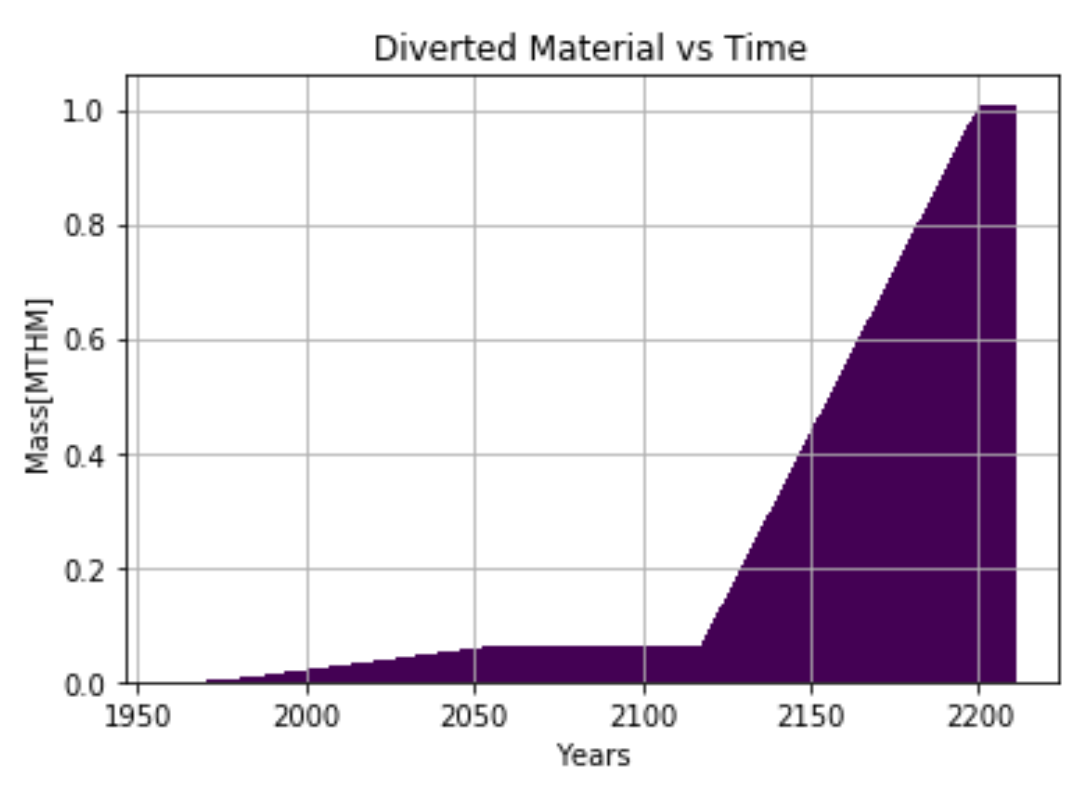
\includegraphics[width=0.9\linewidth]{images/divertmat}
	\caption{A timeseries of diverted material from two Pyre facilities.}
	\label{fig:divertmat}
\end{figure}

\section{Test Cases}

\subsection{PRIDE}

\subsection{INL}

\subsection{ANL}

\section{Sensitivity Analysis}

Sensitivity analysis is an important aspect of this work to know the limits of monitoring these facilities. In this work we use Dakota to alter \Cyclus input files, allowing us to easily
run batches of scenarios. To properly use Dakota with \Cyclus, we must use DCWrapper, which uses python to interface between Dakota and \Cyclus' xml input files. 
Key parameters were run over a range of values for diversion to verify the archetype's capabilities and identify operational ranges. Parameters were selected from the most attractive
sub-processes for diversion, the electrorefiner and electrowinner. These two processes are responsible for the production of Uranium and U/TRU ingots, therefore sensitivity analysis was run
on each of their key parameters: Temperature, Current, Flowrate, Pressure, Stirrer Speed and Reprocessing Time.

\subsection{Temperature}

\begin{figure}
	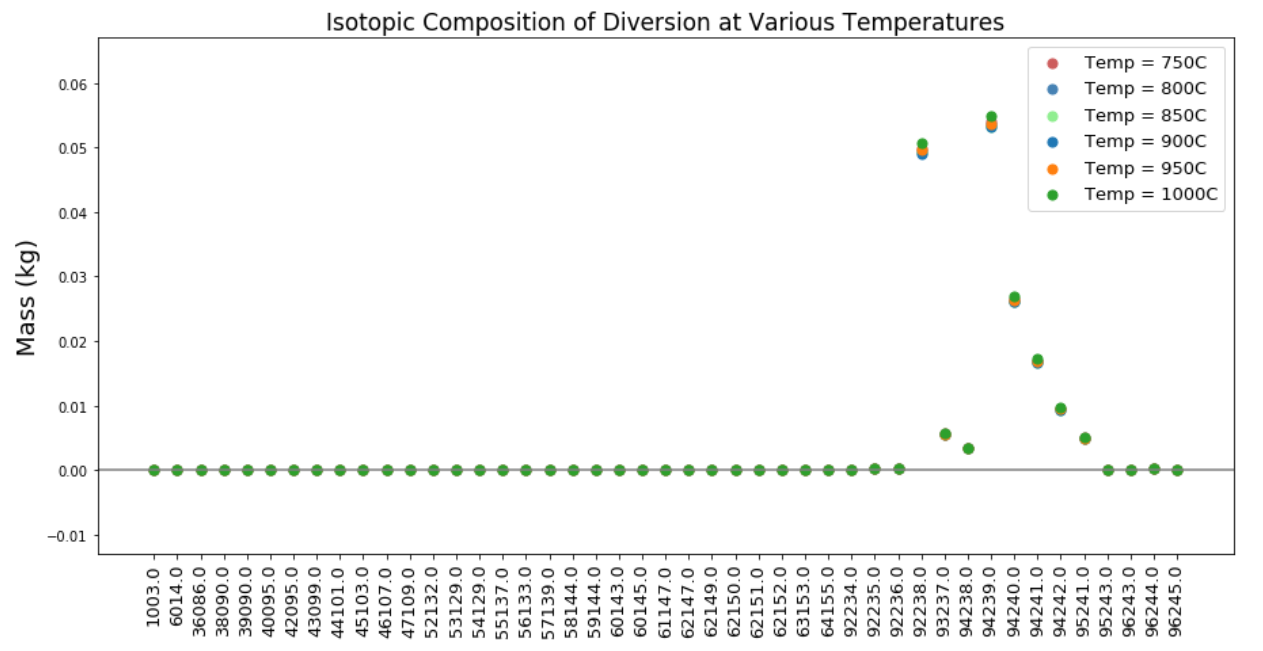
\includegraphics[width=\linewidth]{images/temp-sa-comp}
	\caption{Isotopic composition of the Diverted material stream at various Refiner temperatures.}
	\label{fig:ref-pres-sa}
\end{figure}

\begin{figure}
	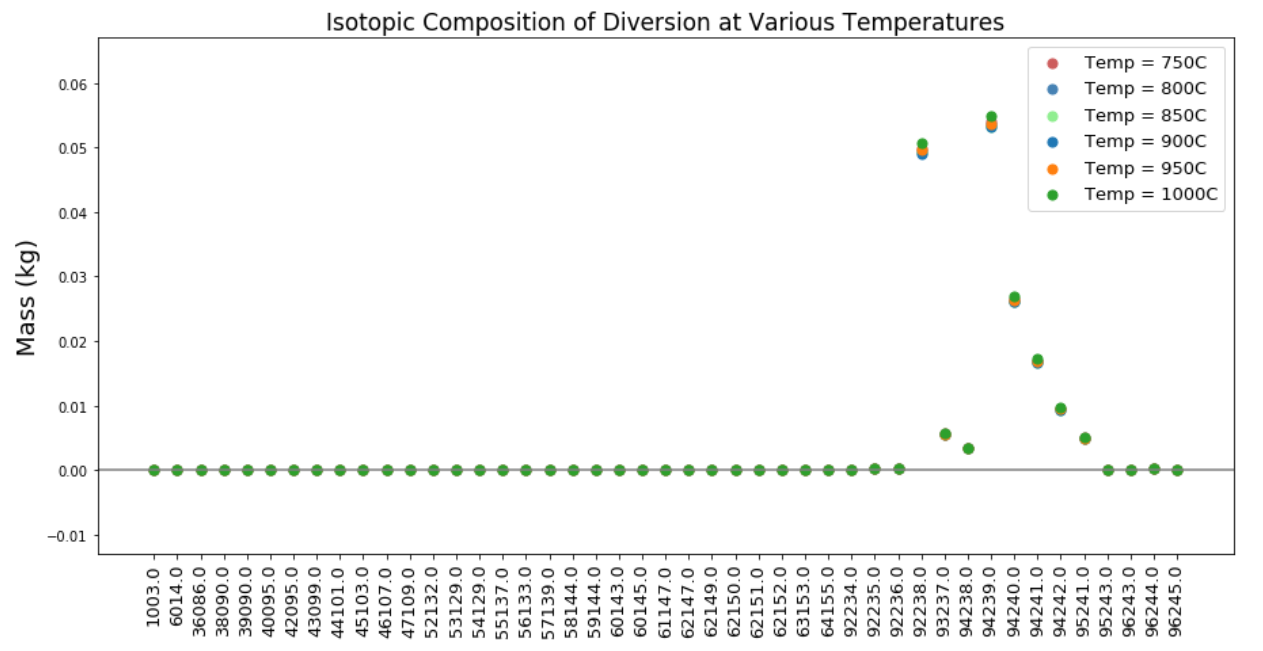
\includegraphics[width=\linewidth]{images/temp-sa-comp}
	\caption{Isotopic composition of the Diverted material stream at various Refiner temperatures.}
	\label{fig:ref-pres-diff}
\end{figure}

\subsection{Current}

\begin{figure}
	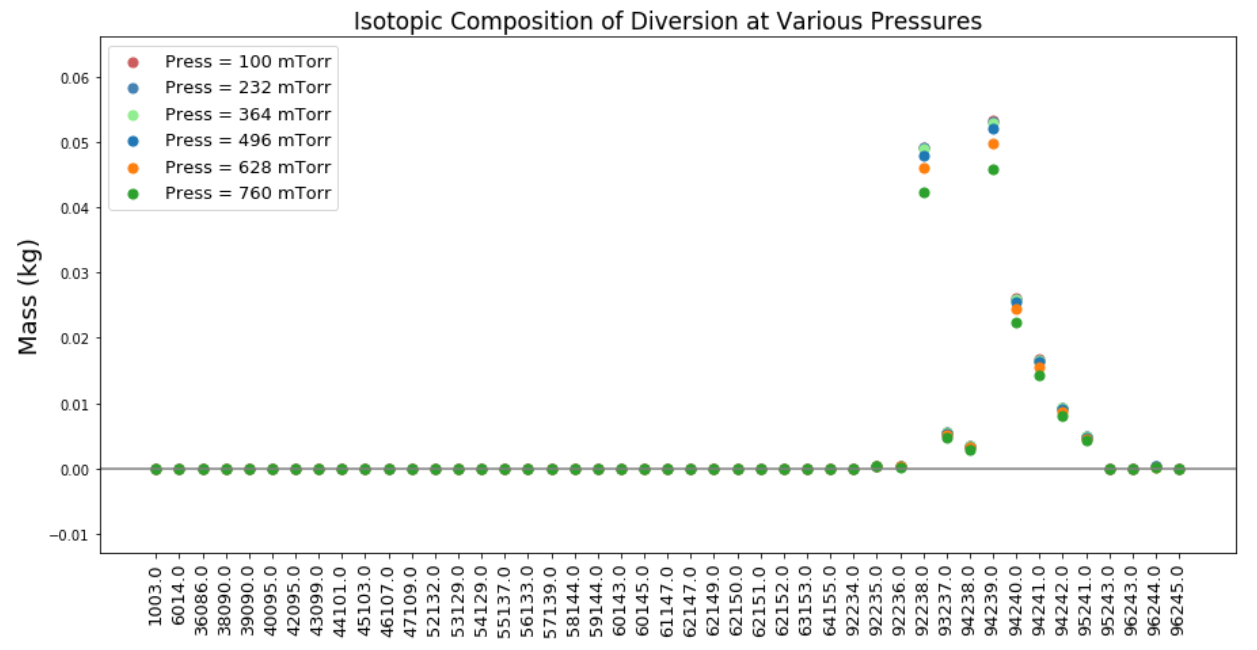
\includegraphics[width=\linewidth]{images/pressure-sa-comp}
	\caption{Isotopic composition of the Diverted material stream at various Electrowinner currents.}
	\label{fig:win-cur-sa}
\end{figure}

\begin{figure}
	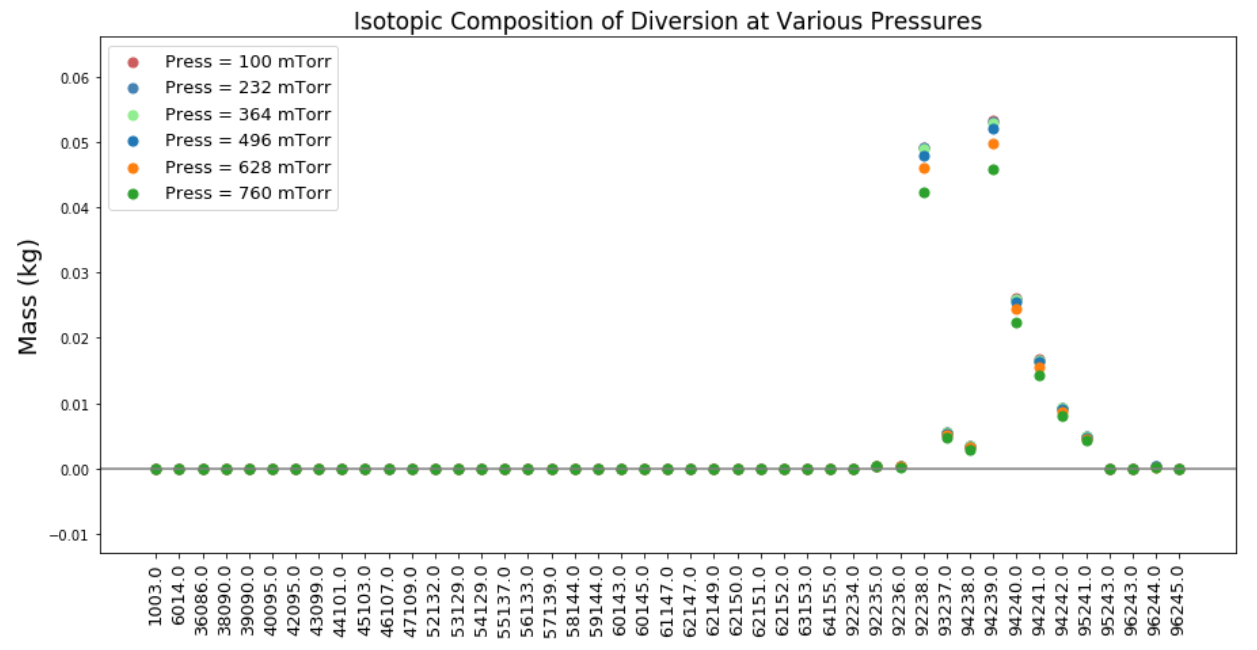
\includegraphics[width=\linewidth]{images/pressure-sa-comp}
	\caption{Isotopic composition of the Diverted material stream at various Electrowinner currents.}
	\label{fig:win-cur-diff}
\end{figure}

\subsection{Flowrate}

\begin{figure}
	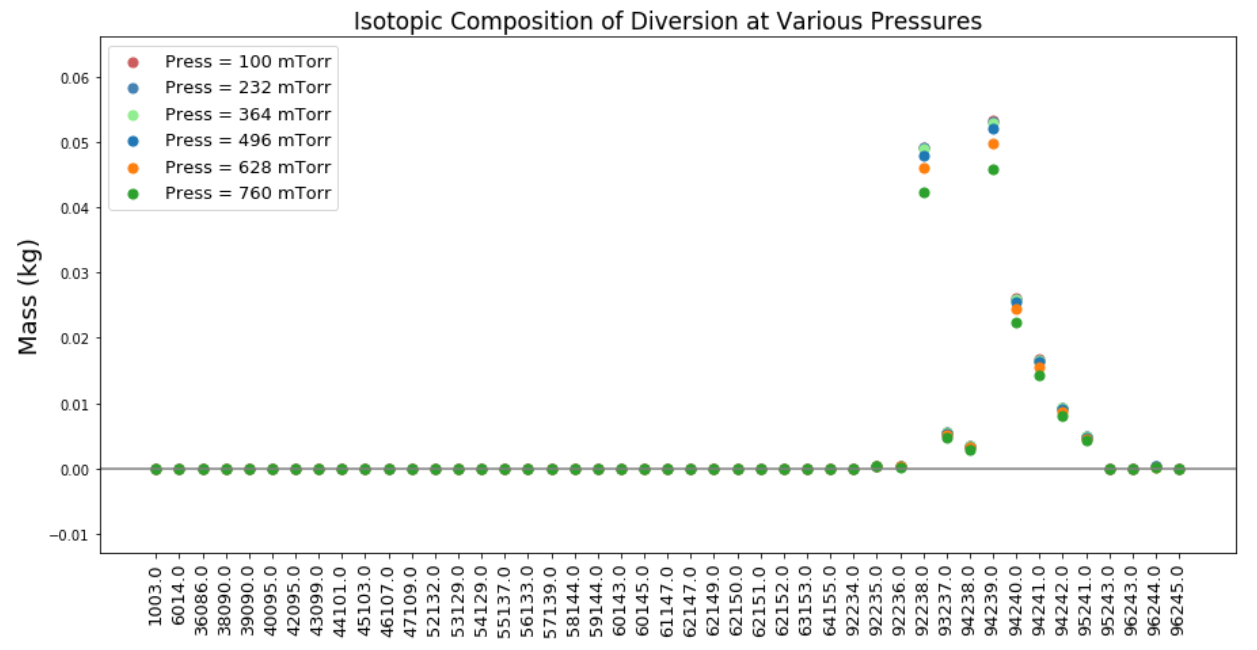
\includegraphics[width=\linewidth]{images/pressure-sa-comp}
	\caption{Isotopic composition of the Diverted material stream at various Electrowinner flowrates.}
	\label{fig:win-flow-sa}
\end{figure}

\begin{figure}
	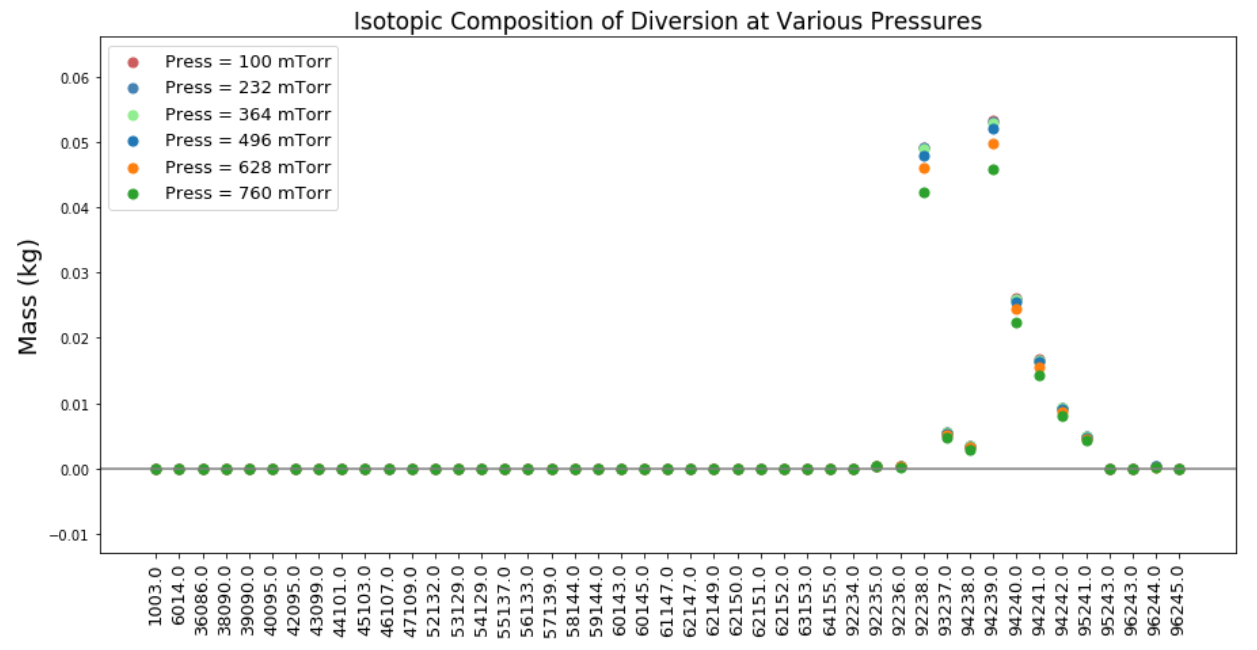
\includegraphics[width=\linewidth]{images/pressure-sa-comp}
	\caption{Isotopic composition of the Diverted material stream at various Electrowinner flowrates.}
	\label{fig:win-flow-diff}
\end{figure}

\subsection{Pressure}

\begin{figure}
	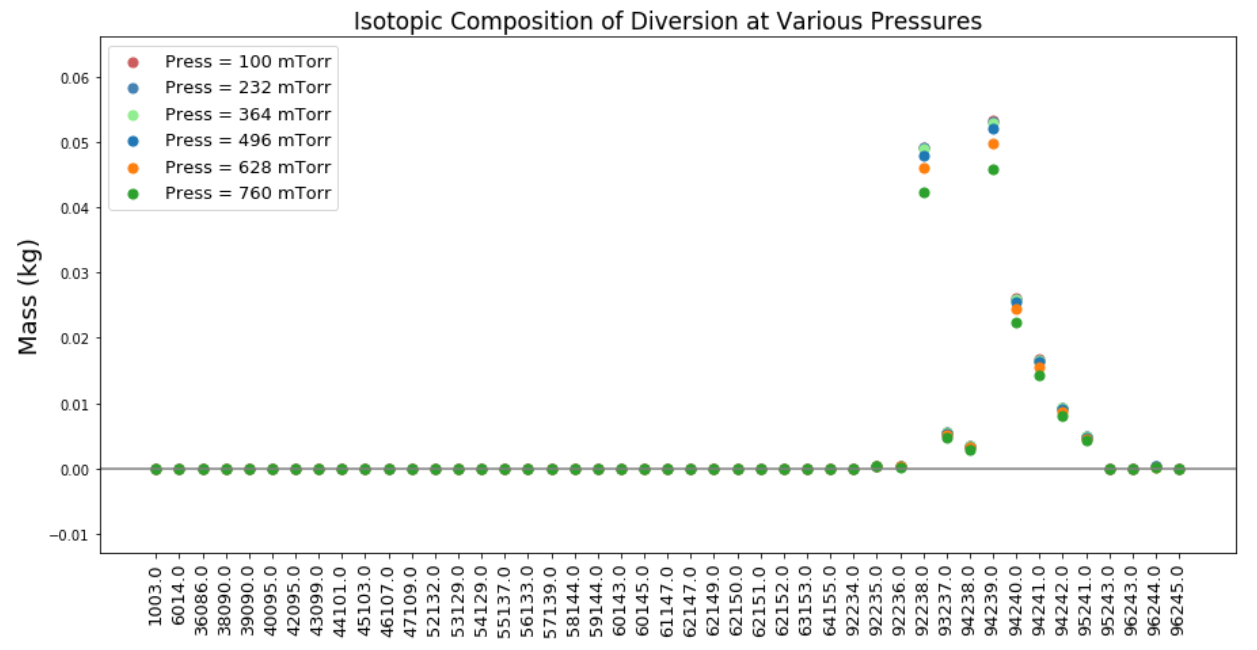
\includegraphics[width=\linewidth]{images/pressure-sa-comp}
	\caption{Isotopic composition of the Diverted material stream at various Refiner pressures.}
	\label{fig:win-cur-sa}
\end{figure}

\begin{figure}
	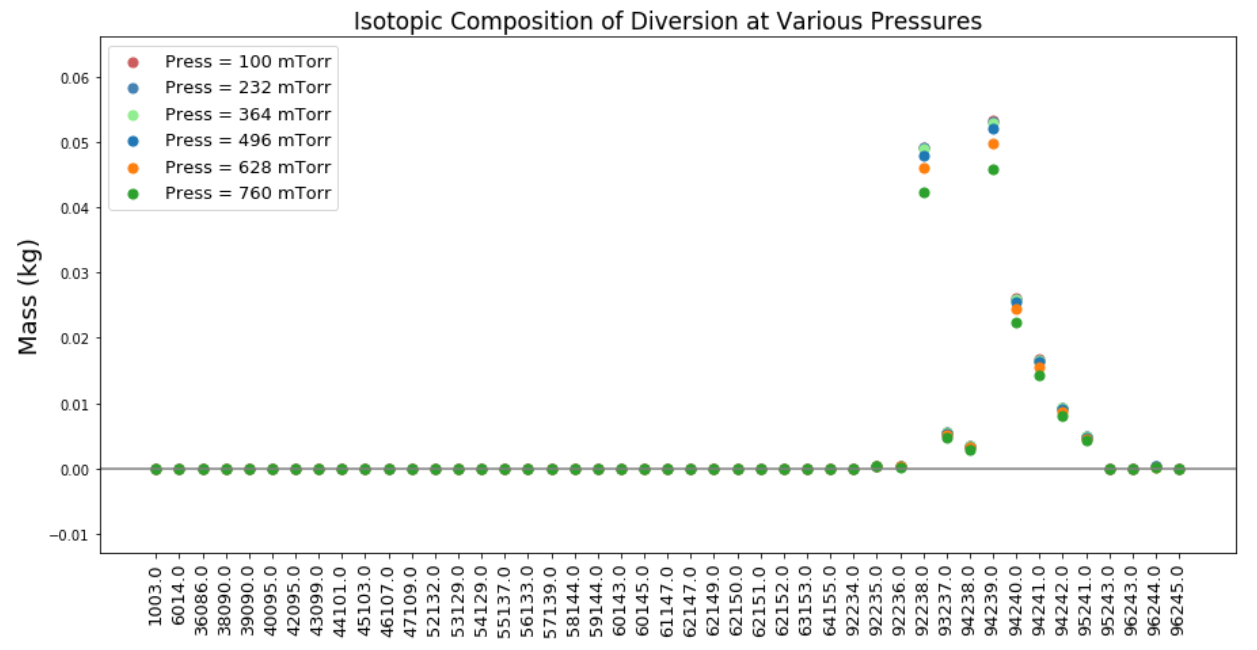
\includegraphics[width=\linewidth]{images/pressure-sa-comp}
	\caption{Isotopic composition of the Diverted material stream at various Refiner pressures.}
	\label{fig:win-cur-diff}
\end{figure}

\subsection{Stirrer Speed}

\begin{figure}
	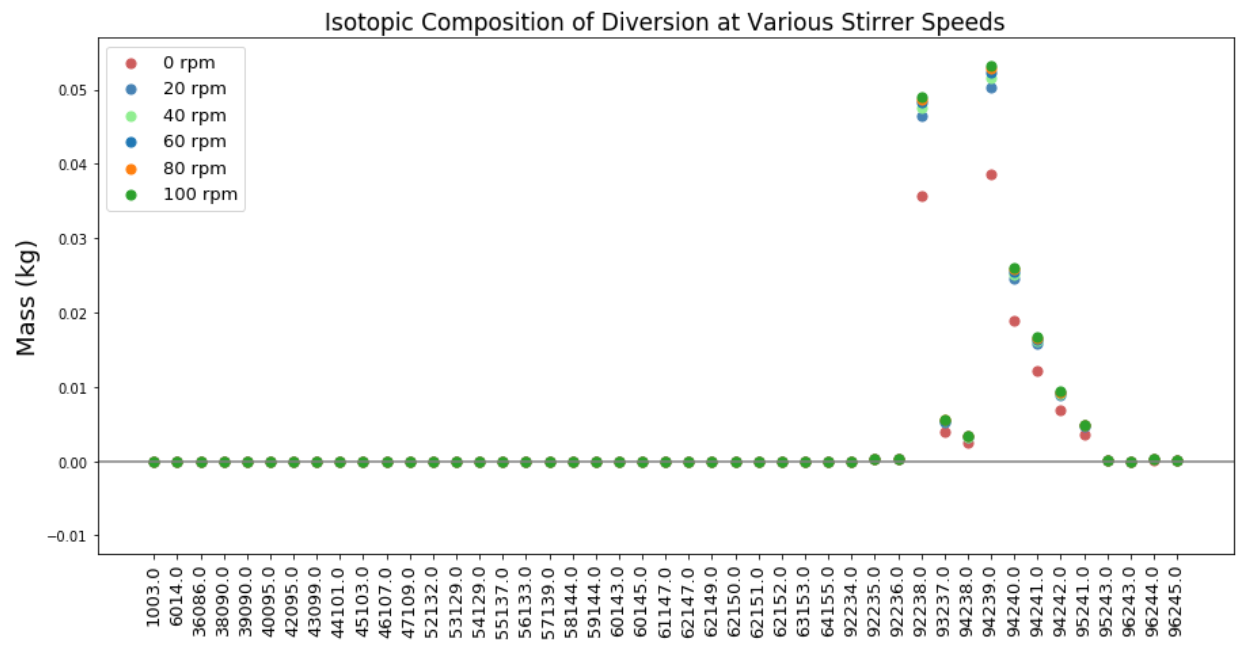
\includegraphics[width=\linewidth]{images/ref-rot-comp}
	\caption{Isotopic composition of the Diverted material stream at various central stirrer speeds.}
	\label{fig:ref-rot-sa}
\end{figure}

\begin{figure}
	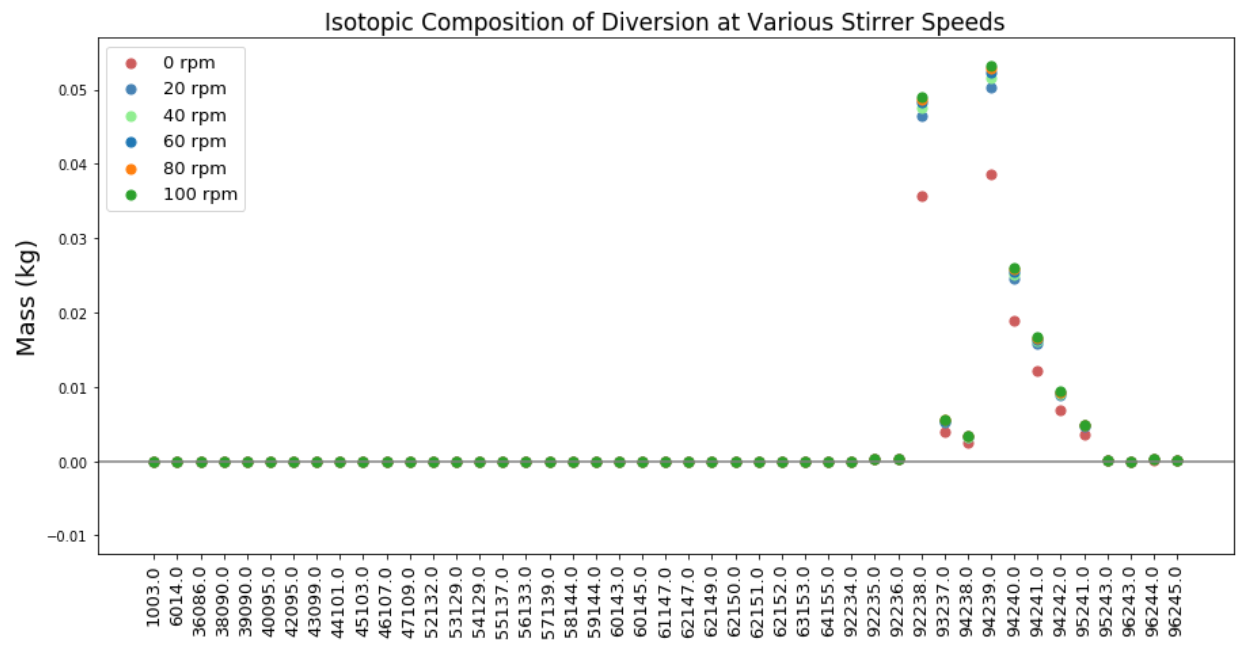
\includegraphics[width=\linewidth]{images/ref-rot-comp}
	\caption{Isotopic composition of the Diverted material stream at various central stirrer speeds.}
	\label{fig:ref-rot-diff}
\end{figure}

\subsection{Reprocessing Time}

\begin{figure}
	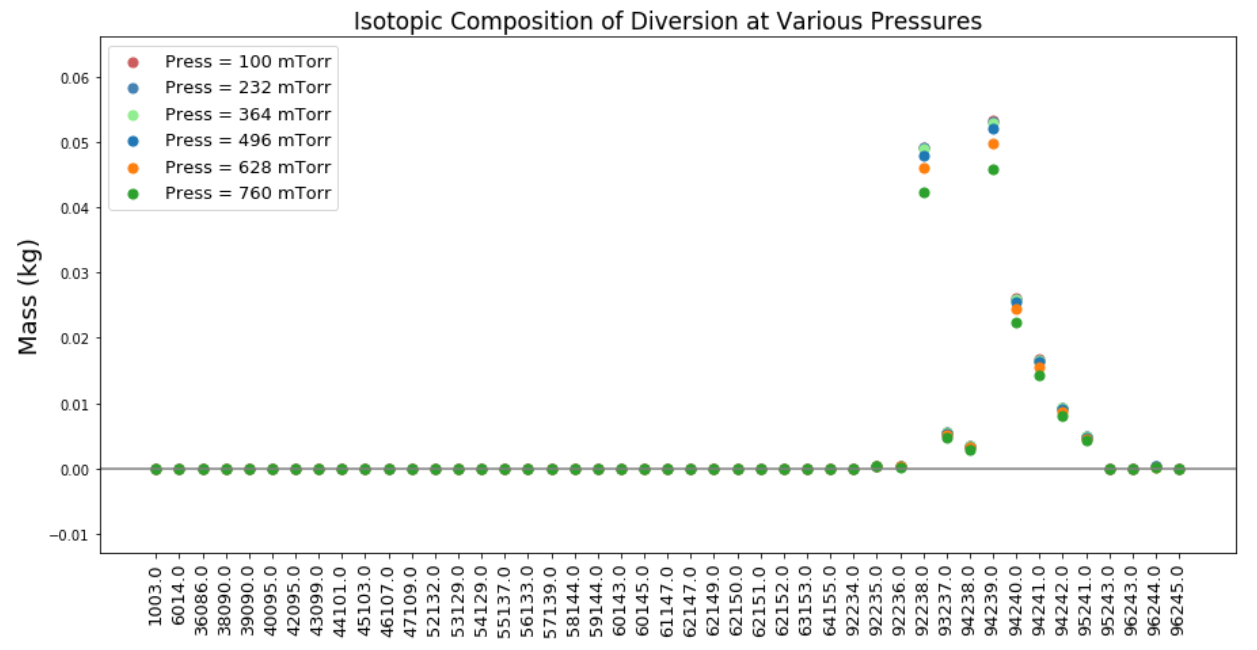
\includegraphics[width=\linewidth]{images/pressure-sa-comp}
	\caption{Isotopic composition of the Diverted material stream at various Electrowinner reprocessing durations.}
	\label{fig:win-time-sa}
\end{figure}

\begin{figure}
	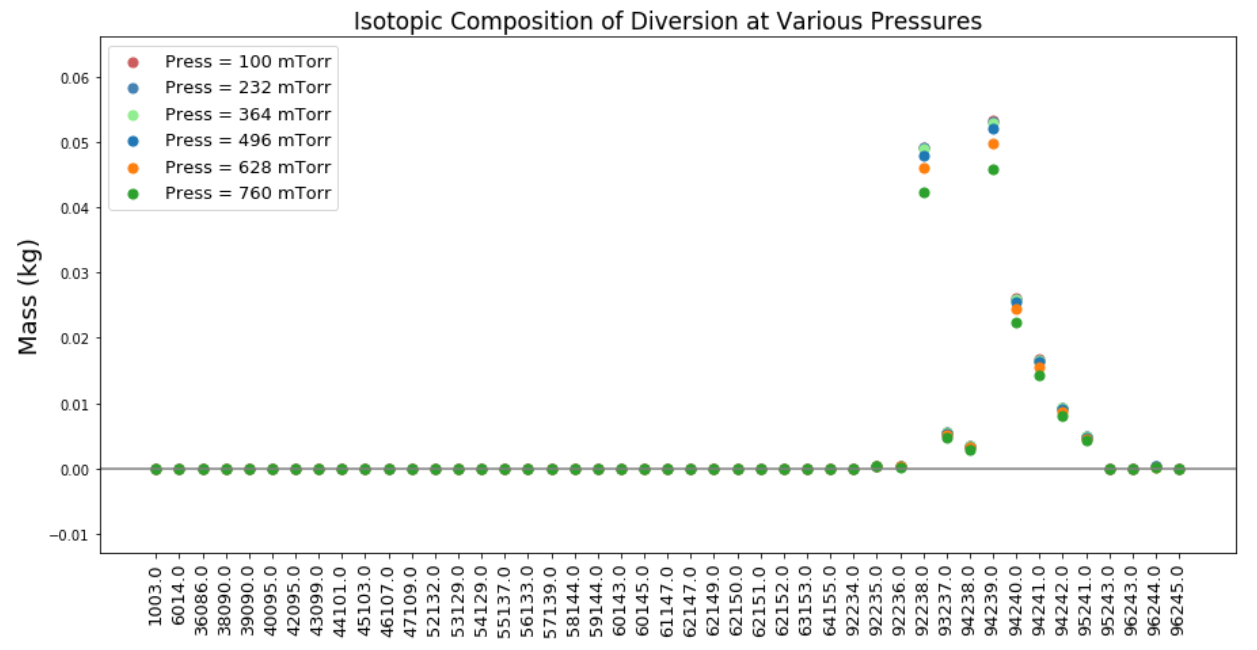
\includegraphics[width=\linewidth]{images/pressure-sa-comp}
	\caption{Isotopic composition of the Diverted material stream at various Electrowinner reprocessing durations.}
	\label{fig:win-time-diff}
\end{figure}